% Generated by ArticleSignalDiagrams. Opaque vector fills only.
\documentclass[10pt,tikz,border=5pt]{standalone}
\usepackage{lmodern}
\usetikzlibrary{fit}
\begin{document}
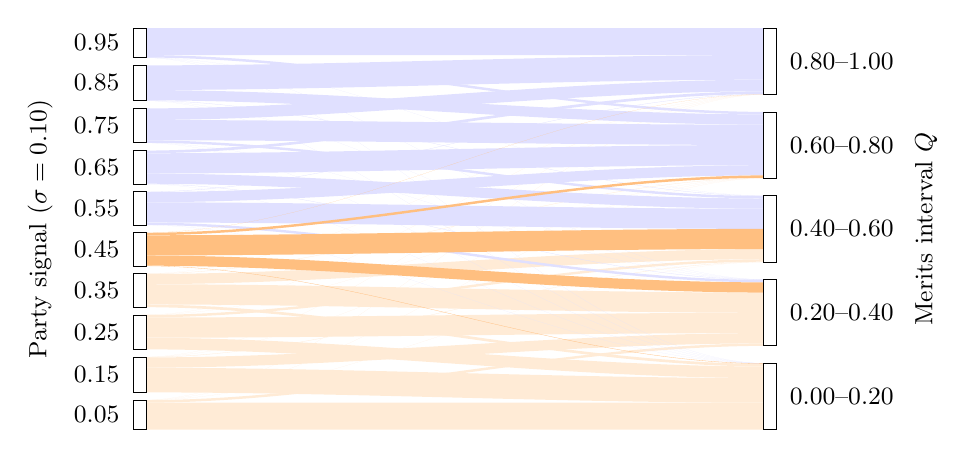
\begin{tikzpicture}[x=1cm,y=1cm,font=\small]\path[fill=orange!16!white,draw=none] (3.3,-5.1) .. controls (6,-5.1) and (8.6,-5.1) .. (11.3,-5.1) -- (11.3,-4.75809) .. controls (8.6,-4.75809) and (6,-4.75809) .. (3.3,-4.75809) -- cycle;
\path[fill=orange!16!white,draw=none] (3.3,-4.75809) .. controls (6,-4.75809) and (8.6,-4.035) .. (11.3,-4.035) -- (11.3,-4.003414) .. controls (8.6,-4.003414) and (6,-4.726505) .. (3.3,-4.726505) -- cycle;
\path[fill=orange!16!white,draw=none] (3.3,-4.726505) .. controls (6,-4.726505) and (8.6,-2.97) .. (11.3,-2.97) -- (11.3,-2.969842) .. controls (8.6,-2.969842) and (6,-4.726347) .. (3.3,-4.726347) -- cycle;
\path[fill=orange!16!white,draw=none] (3.3,-4.726347) .. controls (6,-4.726347) and (8.6,-1.905) .. (11.3,-1.905) -- (11.3,-1.905) .. controls (8.6,-1.905) and (6,-4.726347) .. (3.3,-4.726347) -- cycle;
\path[fill=orange!16!white,draw=none] (3.3,-4.726347) .. controls (6,-4.726347) and (8.6,-0.84) .. (11.3,-0.84) -- (11.3,-0.84) .. controls (8.6,-0.84) and (6,-4.726347) .. (3.3,-4.726347) -- cycle;
\path[fill=orange!16!white,draw=none] (3.3,-4.626347) .. controls (6,-4.626347) and (8.6,-4.75809) .. (11.3,-4.75809) -- (11.3,-4.445106) .. controls (8.6,-4.445106) and (6,-4.313363) .. (3.3,-4.313363) -- cycle;
\path[fill=orange!16!white,draw=none] (3.3,-4.313363) .. controls (6,-4.313363) and (8.6,-4.003414) .. (11.3,-4.003414) -- (11.3,-3.873261) .. controls (8.6,-3.873261) and (6,-4.18321) .. (3.3,-4.18321) -- cycle;
\path[fill=orange!16!white,draw=none] (3.3,-4.18321) .. controls (6,-4.18321) and (8.6,-2.969842) .. (11.3,-2.969842) -- (11.3,-2.96644) .. controls (8.6,-2.96644) and (6,-4.179807) .. (3.3,-4.179807) -- cycle;
\path[fill=orange!16!white,draw=none] (3.3,-4.179807) .. controls (6,-4.179807) and (8.6,-1.905) .. (11.3,-1.905) -- (11.3,-1.904997) .. controls (8.6,-1.904997) and (6,-4.179804) .. (3.3,-4.179804) -- cycle;
\path[fill=orange!16!white,draw=none] (3.3,-4.179804) .. controls (6,-4.179804) and (8.6,-0.84) .. (11.3,-0.84) -- (11.3,-0.84) .. controls (8.6,-0.84) and (6,-4.179804) .. (3.3,-4.179804) -- cycle;
\path[fill=orange!16!white,draw=none] (3.3,-4.079804) .. controls (6,-4.079804) and (8.6,-4.445106) .. (11.3,-4.445106) -- (11.3,-4.297898) .. controls (8.6,-4.297898) and (6,-3.932597) .. (3.3,-3.932597) -- cycle;
\path[fill=orange!16!white,draw=none] (3.3,-3.932597) .. controls (6,-3.932597) and (8.6,-3.873261) .. (11.3,-3.873261) -- (11.3,-3.615942) .. controls (8.6,-3.615942) and (6,-3.675278) .. (3.3,-3.675278) -- cycle;
\path[fill=orange!16!white,draw=none] (3.3,-3.675278) .. controls (6,-3.675278) and (8.6,-2.96644) .. (11.3,-2.96644) -- (11.3,-2.935171) .. controls (8.6,-2.935171) and (6,-3.644008) .. (3.3,-3.644008) -- cycle;
\path[fill=orange!16!white,draw=none] (3.3,-3.644008) .. controls (6,-3.644008) and (8.6,-1.904997) .. (11.3,-1.904997) -- (11.3,-1.904839) .. controls (8.6,-1.904839) and (6,-3.643851) .. (3.3,-3.643851) -- cycle;
\path[fill=orange!16!white,draw=none] (3.3,-3.643851) .. controls (6,-3.643851) and (8.6,-0.84) .. (11.3,-0.84) -- (11.3,-0.84) .. controls (8.6,-0.84) and (6,-3.643851) .. (3.3,-3.643851) -- cycle;
\path[fill=orange!16!white,draw=none] (3.3,-3.543851) .. controls (6,-3.543851) and (8.6,-4.297898) .. (11.3,-4.297898) -- (11.3,-4.263792) .. controls (8.6,-4.263792) and (6,-3.509744) .. (3.3,-3.509744) -- cycle;
\path[fill=orange!16!white,draw=none] (3.3,-3.509744) .. controls (6,-3.509744) and (8.6,-3.615942) .. (11.3,-3.615942) -- (11.3,-3.359195) .. controls (8.6,-3.359195) and (6,-3.252997) .. (3.3,-3.252997) -- cycle;
\path[fill=orange!16!white,draw=none] (3.3,-3.252997) .. controls (6,-3.252997) and (8.6,-2.935171) .. (11.3,-2.935171) -- (11.3,-2.806012) .. controls (8.6,-2.806012) and (6,-3.123838) .. (3.3,-3.123838) -- cycle;
\path[fill=orange!16!white,draw=none] (3.3,-3.123838) .. controls (6,-3.123838) and (8.6,-1.904839) .. (11.3,-1.904839) -- (11.3,-1.901436) .. controls (8.6,-1.901436) and (6,-3.120434) .. (3.3,-3.120434) -- cycle;
\path[fill=orange!16!white,draw=none] (3.3,-3.120434) .. controls (6,-3.120434) and (8.6,-0.84) .. (11.3,-0.84) -- (11.3,-0.839997) .. controls (8.6,-0.839997) and (6,-3.120431) .. (3.3,-3.120431) -- cycle;
\path[fill=blue!12!white,draw=none] (3.3,-2.5) .. controls (6,-2.5) and (8.6,-4.260169) .. (11.3,-4.260169) -- (11.3,-4.260003) .. controls (8.6,-4.260003) and (6,-2.499834) .. (3.3,-2.499834) -- cycle;
\path[fill=blue!12!white,draw=none] (3.3,-2.499834) .. controls (6,-2.499834) and (8.6,-3.229854) .. (11.3,-3.229854) -- (11.3,-3.198564) .. controls (8.6,-3.198564) and (6,-2.468545) .. (3.3,-2.468545) -- cycle;
\path[fill=blue!12!white,draw=none] (3.3,-2.468545) .. controls (6,-2.468545) and (8.6,-2.55) .. (11.3,-2.55) -- (11.3,-2.293988) .. controls (8.6,-2.293988) and (6,-2.212533) .. (3.3,-2.212533) -- cycle;
\path[fill=blue!12!white,draw=none] (3.3,-2.212533) .. controls (6,-2.212533) and (8.6,-1.870146) .. (11.3,-1.870146) -- (11.3,-1.740805) .. controls (8.6,-1.740805) and (6,-2.083192) .. (3.3,-2.083192) -- cycle;
\path[fill=blue!12!white,draw=none] (3.3,-2.083192) .. controls (6,-2.083192) and (8.6,-0.839831) .. (11.3,-0.839831) -- (11.3,-0.836208) .. controls (8.6,-0.836208) and (6,-2.079569) .. (3.3,-2.079569) -- cycle;
\path[fill=blue!12!white,draw=none] (3.3,-1.979569) .. controls (6,-1.979569) and (8.6,-4.260003) .. (11.3,-4.260003) -- (11.3,-4.26) .. controls (8.6,-4.26) and (6,-1.979566) .. (3.3,-1.979566) -- cycle;
\path[fill=blue!12!white,draw=none] (3.3,-1.979566) .. controls (6,-1.979566) and (8.6,-3.198564) .. (11.3,-3.198564) -- (11.3,-3.195161) .. controls (8.6,-3.195161) and (6,-1.976162) .. (3.3,-1.976162) -- cycle;
\path[fill=blue!12!white,draw=none] (3.3,-1.976162) .. controls (6,-1.976162) and (8.6,-2.293988) .. (11.3,-2.293988) -- (11.3,-2.164829) .. controls (8.6,-2.164829) and (6,-1.847003) .. (3.3,-1.847003) -- cycle;
\path[fill=blue!12!white,draw=none] (3.3,-1.847003) .. controls (6,-1.847003) and (8.6,-1.740805) .. (11.3,-1.740805) -- (11.3,-1.484058) .. controls (8.6,-1.484058) and (6,-1.590256) .. (3.3,-1.590256) -- cycle;
\path[fill=blue!12!white,draw=none] (3.3,-1.590256) .. controls (6,-1.590256) and (8.6,-0.836208) .. (11.3,-0.836208) -- (11.3,-0.802102) .. controls (8.6,-0.802102) and (6,-1.556149) .. (3.3,-1.556149) -- cycle;
\path[fill=blue!12!white,draw=none] (3.3,-1.456149) .. controls (6,-1.456149) and (8.6,-4.26) .. (11.3,-4.26) -- (11.3,-4.26) .. controls (8.6,-4.26) and (6,-1.456149) .. (3.3,-1.456149) -- cycle;
\path[fill=blue!12!white,draw=none] (3.3,-1.456149) .. controls (6,-1.456149) and (8.6,-3.195161) .. (11.3,-3.195161) -- (11.3,-3.195003) .. controls (8.6,-3.195003) and (6,-1.455992) .. (3.3,-1.455992) -- cycle;
\path[fill=blue!12!white,draw=none] (3.3,-1.455992) .. controls (6,-1.455992) and (8.6,-2.164829) .. (11.3,-2.164829) -- (11.3,-2.13356) .. controls (8.6,-2.13356) and (6,-1.424722) .. (3.3,-1.424722) -- cycle;
\path[fill=blue!12!white,draw=none] (3.3,-1.424722) .. controls (6,-1.424722) and (8.6,-1.484058) .. (11.3,-1.484058) -- (11.3,-1.226739) .. controls (8.6,-1.226739) and (6,-1.167403) .. (3.3,-1.167403) -- cycle;
\path[fill=blue!12!white,draw=none] (3.3,-1.167403) .. controls (6,-1.167403) and (8.6,-0.802102) .. (11.3,-0.802102) -- (11.3,-0.654894) .. controls (8.6,-0.654894) and (6,-1.020196) .. (3.3,-1.020196) -- cycle;
\path[fill=blue!12!white,draw=none] (3.3,-0.920196) .. controls (6,-0.920196) and (8.6,-4.26) .. (11.3,-4.26) -- (11.3,-4.26) .. controls (8.6,-4.26) and (6,-0.920196) .. (3.3,-0.920196) -- cycle;
\path[fill=blue!12!white,draw=none] (3.3,-0.920196) .. controls (6,-0.920196) and (8.6,-3.195003) .. (11.3,-3.195003) -- (11.3,-3.195) .. controls (8.6,-3.195) and (6,-0.920193) .. (3.3,-0.920193) -- cycle;
\path[fill=blue!12!white,draw=none] (3.3,-0.920193) .. controls (6,-0.920193) and (8.6,-2.13356) .. (11.3,-2.13356) -- (11.3,-2.130158) .. controls (8.6,-2.130158) and (6,-0.91679) .. (3.3,-0.91679) -- cycle;
\path[fill=blue!12!white,draw=none] (3.3,-0.91679) .. controls (6,-0.91679) and (8.6,-1.226739) .. (11.3,-1.226739) -- (11.3,-1.096586) .. controls (8.6,-1.096586) and (6,-0.786637) .. (3.3,-0.786637) -- cycle;
\path[fill=blue!12!white,draw=none] (3.3,-0.786637) .. controls (6,-0.786637) and (8.6,-0.654894) .. (11.3,-0.654894) -- (11.3,-0.34191) .. controls (8.6,-0.34191) and (6,-0.473653) .. (3.3,-0.473653) -- cycle;
\path[fill=blue!12!white,draw=none] (3.3,-0.373653) .. controls (6,-0.373653) and (8.6,-4.26) .. (11.3,-4.26) -- (11.3,-4.26) .. controls (8.6,-4.26) and (6,-0.373653) .. (3.3,-0.373653) -- cycle;
\path[fill=blue!12!white,draw=none] (3.3,-0.373653) .. controls (6,-0.373653) and (8.6,-3.195) .. (11.3,-3.195) -- (11.3,-3.195) .. controls (8.6,-3.195) and (6,-0.373653) .. (3.3,-0.373653) -- cycle;
\path[fill=blue!12!white,draw=none] (3.3,-0.373653) .. controls (6,-0.373653) and (8.6,-2.130158) .. (11.3,-2.130158) -- (11.3,-2.13) .. controls (8.6,-2.13) and (6,-0.373495) .. (3.3,-0.373495) -- cycle;
\path[fill=blue!12!white,draw=none] (3.3,-0.373495) .. controls (6,-0.373495) and (8.6,-1.096586) .. (11.3,-1.096586) -- (11.3,-1.065) .. controls (8.6,-1.065) and (6,-0.34191) .. (3.3,-0.34191) -- cycle;
\path[fill=blue!12!white,draw=none] (3.3,-0.34191) .. controls (6,-0.34191) and (8.6,-0.34191) .. (11.3,-0.34191) -- (11.3,0) .. controls (8.6,0) and (6,0) .. (3.3,0) -- cycle;
\path[fill=orange!50!white,draw=none] (3.3,-3.020431) .. controls (6,-3.020431) and (8.6,-4.263792) .. (11.3,-4.263792) -- (11.3,-4.260169) .. controls (8.6,-4.260169) and (6,-3.016808) .. (3.3,-3.016808) -- cycle;
\path[fill=orange!50!white,draw=none] (3.3,-3.016808) .. controls (6,-3.016808) and (8.6,-3.359195) .. (11.3,-3.359195) -- (11.3,-3.229854) .. controls (8.6,-3.229854) and (6,-2.887467) .. (3.3,-2.887467) -- cycle;
\path[fill=orange!50!white,draw=none] (3.3,-2.887467) .. controls (6,-2.887467) and (8.6,-2.806012) .. (11.3,-2.806012) -- (11.3,-2.55) .. controls (8.6,-2.55) and (6,-2.631455) .. (3.3,-2.631455) -- cycle;
\path[fill=orange!50!white,draw=none] (3.3,-2.631455) .. controls (6,-2.631455) and (8.6,-1.901436) .. (11.3,-1.901436) -- (11.3,-1.870146) .. controls (8.6,-1.870146) and (6,-2.600166) .. (3.3,-2.600166) -- cycle;
\path[fill=orange!50!white,draw=none] (3.3,-2.600166) .. controls (6,-2.600166) and (8.6,-0.839997) .. (11.3,-0.839997) -- (11.3,-0.839831) .. controls (8.6,-0.839831) and (6,-2.6) .. (3.3,-2.6) -- cycle;
\coordinate (axis-midline-0) at (0,-2.55);
\path[fill=white,draw=black,line width=0.3pt] (3.22,-5.1) rectangle (3.38,-4.726347);
\node[anchor=east,fill=white,inner sep=2pt] (bucket-0-0-0) at (3.12,-4.913174) {0.05};
\path[fill=white,draw=black,line width=0.3pt] (3.22,-4.626347) rectangle (3.38,-4.179804);
\node[anchor=east,fill=white,inner sep=2pt] (bucket-0-0-1) at (3.12,-4.403075) {0.15};
\path[fill=white,draw=black,line width=0.3pt] (3.22,-4.079804) rectangle (3.38,-3.643851);
\node[anchor=east,fill=white,inner sep=2pt] (bucket-0-0-2) at (3.12,-3.861827) {0.25};
\path[fill=white,draw=black,line width=0.3pt] (3.22,-3.543851) rectangle (3.38,-3.120431);
\node[anchor=east,fill=white,inner sep=2pt] (bucket-0-0-3) at (3.12,-3.332141) {0.35};
\path[fill=white,draw=black,line width=0.3pt] (3.22,-3.020431) rectangle (3.38,-2.6);
\node[anchor=east,fill=white,inner sep=2pt] (bucket-0-0-4) at (3.12,-2.810216) {0.45};
\path[fill=white,draw=black,line width=0.3pt] (3.22,-2.5) rectangle (3.38,-2.079569);
\node[anchor=east,fill=white,inner sep=2pt] (bucket-0-0-5) at (3.12,-2.289784) {0.55};
\path[fill=white,draw=black,line width=0.3pt] (3.22,-1.979569) rectangle (3.38,-1.556149);
\node[anchor=east,fill=white,inner sep=2pt] (bucket-0-0-6) at (3.12,-1.767859) {0.65};
\path[fill=white,draw=black,line width=0.3pt] (3.22,-1.456149) rectangle (3.38,-1.020196);
\node[anchor=east,fill=white,inner sep=2pt] (bucket-0-0-7) at (3.12,-1.238173) {0.75};
\path[fill=white,draw=black,line width=0.3pt] (3.22,-0.920196) rectangle (3.38,-0.473653);
\node[anchor=east,fill=white,inner sep=2pt] (bucket-0-0-8) at (3.12,-0.696925) {0.85};
\path[fill=white,draw=black,line width=0.3pt] (3.22,-0.373653) rectangle (3.38,0);
\node[anchor=east,fill=white,inner sep=2pt] (bucket-0-0-9) at (3.12,-0.186826) {0.95};
\node[fit=(bucket-0-0-0) (bucket-0-0-1) (bucket-0-0-2) (bucket-0-0-3) (bucket-0-0-4) (bucket-0-0-5) (bucket-0-0-6) (bucket-0-0-7) (bucket-0-0-8) (bucket-0-0-9),inner sep=0pt] (source-labels-0) {};
\coordinate (axis-title-0-0) at (source-labels-0.west |- axis-midline-0);
\node[rotate=90,anchor=south,inner sep=0pt] at ([xshift=-0.18cm]axis-title-0-0) {Party signal ($\sigma=0.10$)};
\path[fill=white,draw=black,line width=0.3pt] (11.22,-5.1) rectangle (11.38,-4.26);
\node[anchor=west,fill=white,inner sep=2pt] (bucket-0-1-0) at (11.48,-4.68) {0.00--0.20};
\path[fill=white,draw=black,line width=0.3pt] (11.22,-4.035) rectangle (11.38,-3.195);
\node[anchor=west,fill=white,inner sep=2pt] (bucket-0-1-1) at (11.48,-3.615) {0.20--0.40};
\path[fill=white,draw=black,line width=0.3pt] (11.22,-2.97) rectangle (11.38,-2.13);
\node[anchor=west,fill=white,inner sep=2pt] (bucket-0-1-2) at (11.48,-2.55) {0.40--0.60};
\path[fill=white,draw=black,line width=0.3pt] (11.22,-1.905) rectangle (11.38,-1.065);
\node[anchor=west,fill=white,inner sep=2pt] (bucket-0-1-3) at (11.48,-1.485) {0.60--0.80};
\path[fill=white,draw=black,line width=0.3pt] (11.22,-0.84) rectangle (11.38,0);
\node[anchor=west,fill=white,inner sep=2pt] (bucket-0-1-4) at (11.48,-0.42) {0.80--1.00};
\node[fit=(bucket-0-1-0) (bucket-0-1-1) (bucket-0-1-2) (bucket-0-1-3) (bucket-0-1-4),inner sep=0pt] (destination-labels-0) {};
\coordinate (axis-title-0-1) at (destination-labels-0.east |- axis-midline-0);
\node[rotate=90,anchor=north,inner sep=0pt] at ([xshift=0.18cm]axis-title-0-1) {Merits interval $Q$};
\end{tikzpicture}
\end{document}

